\documentclass[a4paper,11pt]{article}
\usepackage[T1]{fontenc}

%opening
\title{\texttt{fcc\_analyzer\_PyQt4}: a PyQt4 GUI to visualize \fcc\ output}
\date{\textsc{Version: 0.1}\\\today}
\author{Javier Cerezo\\\texttt{j.cerezo@pi.iccom.cnr.it}}

% Margins
\textheight 22.0cm \textwidth 14.7cm \oddsidemargin 1cm
\evensidemargin 1cm \topmargin -0.25cm

%Packages
\usepackage{graphics}
\usepackage[pdftex]{graphicx}

\usepackage{amsmath}
\usepackage{amssymb}
\usepackage{color}
\usepackage{xcolor}


\begin{document}
\setlength{\parskip}{0.5em}
\newcommand{\fcc}{$\mathcal{FC}$\textit{classes}}

\maketitle

\section{Description}
\texttt{fcc\_analyzer\_PyQt4} is a graphical user interface (GUI) written in python and relying in the PyQt4 and matplotlib libraries that reads the output from \fcc\ (for a TI calculation), namely fort.21 (assignments) and fort.22 (spectral histogram).

\section{Installation}

\subsection{Precompiled binary}
A binary file generated with \texttt{pyinstaller} is provided. It is compatible with 64-bit Linux systems. The GLIBC version $\geq$2.17 is required.

\subsection{Python source. Requirements}
The source can be run directly as a python script. A \texttt{python} (version 2.7) interpreter in required, along with the following modules (the minimum version tested in included):

\begin{itemize}
 \item \texttt{matplotlib} (version $\geq1.4.2$)
 \item \texttt{numpy} (version $\geq1.9.1$)
 \item \texttt{PyQt4} (version $\geq4.10.4$)
\end{itemize}

\clearpage

\section{Running the application}

\subsection{Launch the application}
The application need to be invoked in the folder were the fort.21 and fort.22 files that will be analysed reside, with the following syntax:\\

\texttt{fcc\_analyzer\_PyQt4 [flags]}\\

The following flags are supported:

\begin{tabular}{lll}
 \texttt{-type (abs|emi|ecd|cpl)}     && \begin{minipage}[t]{0.65\textwidth}
                                          Type of {\fcc} calculation performed.
                                         \end{minipage}\\\\
 \texttt{-maxC N}                     && \begin{minipage}[t]{0.65\textwidth}
                                          Maximum class to by loaded (\texttt{N}$\leq7$).
                                         \end{minipage}\\\\
 \texttt{-h}                          && \begin{minipage}[t]{0.65\textwidth}
                                          Show help.
                                         \end{minipage}\\\\
\end{tabular}

\subsection{Using the application}
The GUI consists of the following parts:

\begin{figure}[h!]
\begin{center}
  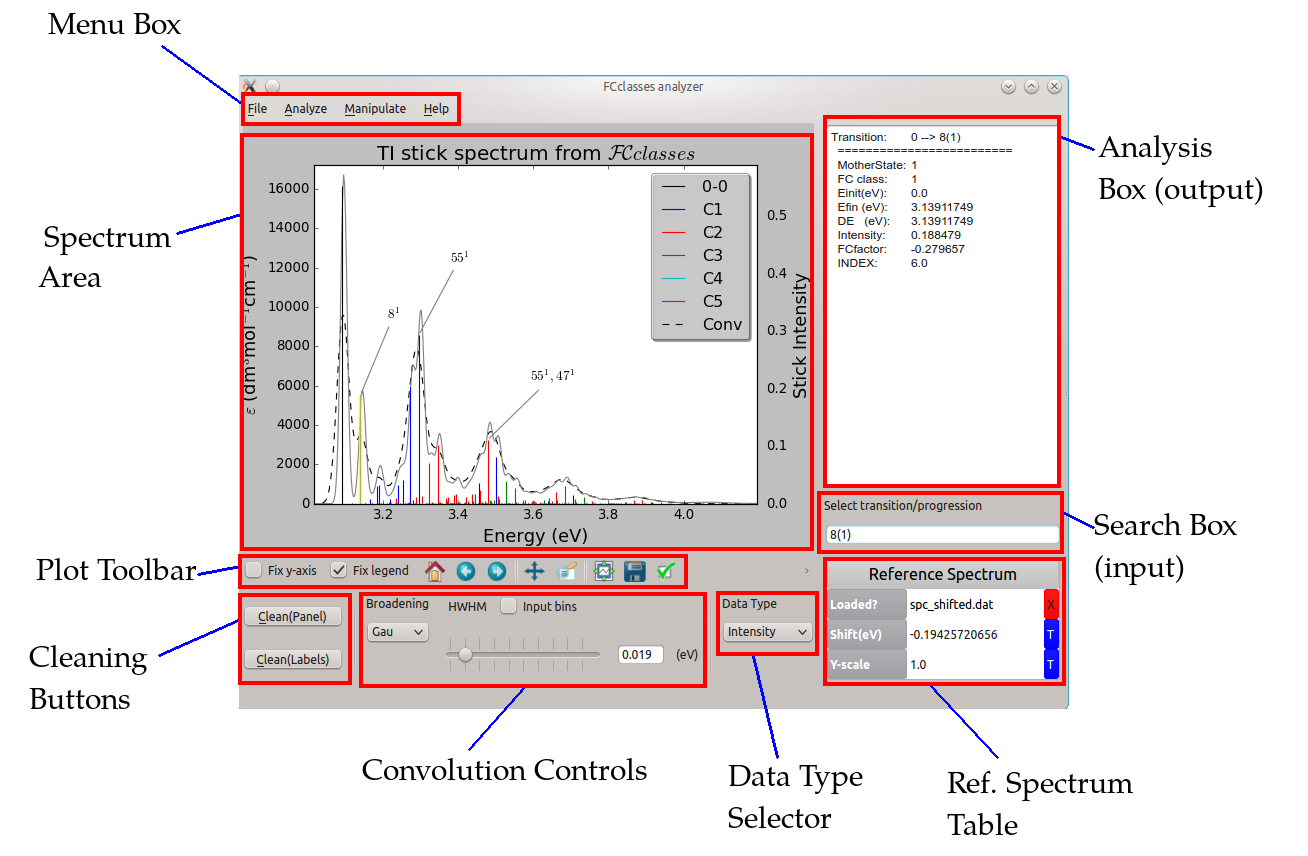
\includegraphics[width=15cm]{figs/fcc_analyzer_screeshot.png}
\end{center}
\caption{Screenshot of \texttt{fcc\_analyzer\_PyQt4} highlighting the different parts.}
\end{figure}

The interaction and analysis of the simulated spectrum are performed with the different widgets in the plot. Below, the different parts are described.

\subsubsection{Menu Box}
\begin{itemize}
 \item File
 \begin{itemize}
  \item Save plot: save plot to a png file.
  \item Export to xmgrace: export plot data (including labels) to xmgrace file
  \item Import plot: Load reference spectrum to the Spectrum Area. Units: (eV|cm$^{-1}$|nm).
 \end{itemize}

 \item Analyse
 \begin{itemize}
  \item Momenta: compute momenta of the convoluted and write to the Analysis Box.
 \end{itemize}

 \item Manipulate
 \begin{itemize}
  \item Shift to simulated: shift reference spectrum (if loaded) to match the convoluted spectrum.
  \item Scale to convoluted: scale reference spectrum (if loaded) to match the convoluted spectrum.
 \end{itemize}
\end{itemize}
 
\subsubsection{Spectrum Area}
This area is interactive. The following actions are possible:
\begin{itemize}
 \item Right-mouse click on a stick: highlight and get info about the transition (written into Analysis Box).
 \item Left-mouse click on a stick: add label over the stick
 \item Right-mouse click on a label: drag the label
 \item Right-mouse click on a legend line: activate/deactivate plot
 \item Press ``+''/``-'' keys to browse back and forward between highlighted stick
\end{itemize}

\subsubsection{Analysis Box}
In this box, the information about the highlighted transitions is shown, as well as the analysis of the momenta. This box is not editable, but the info can be copied.

\subsubsection{Search Box}
Selector of transitions. The general syntax is the following:

{
\scriptsize
\texttt{Mode1'(Quanta1'),Mode2'(Quanta2')... {-}{-}> Mode1(Quanta1),Mode2(Quanta2)...}
}\\

where \texttt{Mode1'(Quanta1')} refer to mode \texttt{Mode1'} in the initial state that is excited \texttt{Quanta1'} quanta, and \texttt{Mode1(Quanta1)} are the equivalent entities for the final state.

The ground vibrational state is represented by a zero (\texttt{0}). When the initial state is in the ground state, the initial part, \texttt{0{-}{-}>} can be omitted. Some examples:

\begin{itemize}
 \item \texttt{8(1),9(2)}: select the transition from the ground initial state to the final state where mode 8 is excited 1 quantum and mode 9 is excited 2 quanta.
 \item \texttt{0{-}{-}>8(1),9(2)}: same as above
 \item \texttt{8(1){-}{-}>0}: select transition from initial state excited 1 quantum on mode 8 to the final ground state.
 \item \texttt{0{-}{-}>0}: select 0-0 transition
\end{itemize}

To select a progression in the final state, use \texttt{P} instead of the number of quanta. This keyword can only be used for one mode in the same selection. Some examples:

\begin{itemize}
 \item \texttt{8(p)}: select progression of mode 8 in the final state.
 \item \texttt{0{-}{-}>8(p),9(2)}: select progression of mode 8 in the final state when, simultaneously, mode 9 is excited 2 quanta.
 \item \texttt{1(1){-}{-}>8(p)}: select progression of mode 8 in the final state, starting from the initial state where mode 1 is excited one quantum.
\end{itemize}

\subsubsection{Plot Toolbar}
This is formed by two check boxes and the standard matplotlib toolbar with PyQt4 back-end. The check boxes are:
\begin{itemize}
 \item Fix y-axis: whether or not scale y-axis when the convolution or the data type are updated.
 \item Fix legend: whether the legend can be displaced with the mouse of not.
\end{itemize}

The matplotlib toolbar include:
\begin{itemize}
 \item 
\includegraphics[width=0.5cm]{figs/butt_zoom.jpg}: zoom into (left mouse click) or out (right mouse click) a rectangle.
 \item 
\includegraphics[width=0.5cm]{figs/butt_move.jpg}: move the spectrum (left mouse click) or zoom (right mouse click).
 \item 
\includegraphics[width=0.5cm]{figs/butt_save.jpg}: export image.
 \item 
\includegraphics[width=0.5cm]{figs/butt_edit.jpg}: customize axes properties.
\end{itemize}

\subsubsection{Cleaning Buttons}
\begin{itemize}
 \item Clean(Panel): remove highlight on transitions and clear the analysis box.
 \item Clean(Labels): clear all labels added to the spectrum
\end{itemize}

\subsubsection{Convolution Controls}
\begin{itemize}
 \item Broadening selector [Gau|Lor]: type of broadening function
 \item HWHM slider and box: set the HWHM of the broadening function
 \item Input bins check box: use the bins given in the input fort.22 file. Otherwise, a new histogram with only 1000 bins is used (which is faster).
\end{itemize}

\subsubsection{Data Type Selector}
Select the type of spectrum: [Intensity|Lineshape].

\subsubsection{Ref. Spectrum Table}
Information about the reference spectrum (loaded with File->Import plot).

\begin{itemize}
 \item Loaded?: whether reference spectrum is loaded. If so the file name is shown. The red button with the cross deletes the reference spectrum.
 \item Shift(eV): shift applied to the reference spectrum (in eV). This box is editable. The value always refer to the originally loaded value, unless the blue T button is pressed, which reset the reference value to the current one.
 \item Y-scale: scaling applied to the reference spectrum Y-axis. This box is editable. The value always refer to the originally loaded value, unless the blue T button is pressed, which reset the reference value to the current one.
\end{itemize}


\end{document}
